\chapter{Introducción Específica} % Main chapter title

\label{Chapter2}
En este capítulo se presenta CIAABOT con más detalle, incluyendo especificaciones técnicas sobre la plataforma utilizada. Se establecen los requerimientos planteados y la planificación para el desarrollo del trabajo.

\section{CIAABOT: Partes componentes}
\label{sec:ciaabot:partes}
Se planteó que para lograr los objetivos propuestos, la plataforma debería estar formada por tres partes fundamentales, que funcionarían complementadas para armar un ecosistema CIAABOT, como está esquematizado en la figura \ref{fig:ciaabot:partes}. A continuación se describirá cada uno de ellos.

\begin{center}
    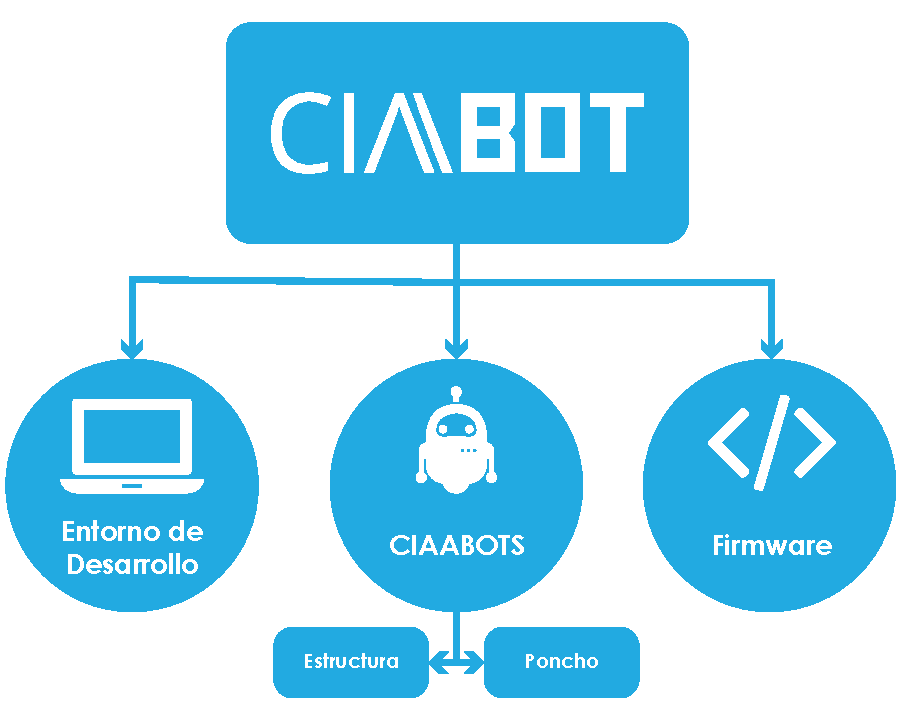
\includegraphics[scale=.8]{./Figures/ciaabot-partes.pdf}
    \label{fig:ciaabot:partes}
    \captionof{figure}{Diagrama de las partes que componen CIAABOT.}
\end{center}


\subsection{Entorno de desarrollo integrado}
\label{subsec:ide}
Un IDE (\emph{Integrated Development Environment}, Entorno de Desarrollo Integrado) es un software que incluye varias herramientas para asistir a los desarrolladores con su trabajo. Generalmente incluye algún editor para el código, herramientas de construcción o compilación automáticas, programación de la plataforma y posible depuración.

El CIAABOT-IDE es el centro del trabajo de los usuarios. Aquí plasman sus ideas y soluciones a problemas planteados. Esto lo hacen por medio de un editor de código en el que utilizan bloques predefinidos y no texto, como se observa en la figura \ref{fig:ciaabot:ide}. Arrastrando e interconectando los mismos logran definir la lógica para su programa.

Una opción interesante para remarcar es la salida de código en C. Cada vez que se modifica el diagrama de bloques, el código en C producido se modifica en tiempo real. Esto es muy útil para gente que pretende aprender a programar en C, ya que ve de manera directa cómo afecta cada bloque a las líneas de código y puede apreciar las equivalencias.

La plataforma también permite compilar y luego descargar el código generado en la placa solamente conectándola por USB.

Una vez que se finalizó el trabajo se puede guardar el proyecto en un archivo \emph{.cbp} que contiene la estructura de bloques en la que se estuvo trabajando, junto con las opciones adicionales del proyecto. Este archivo puede ser compartido y abierto en otra PC para ser reutilizado o modificado y guardado nuevamente.

Otra de las opciones que fue publicada en la última versión de CIAABOT-IDE (v0.0.8) es la de seleccionar los directorios de búsqueda para el toolchain. Las aplicaciones necesarias para todos los sistemas operativos son dos: El compilador arm-none-eabi-gcc y el debugger openOCD. Adicionalmente, en Windows se requieren otros ejecutables como make, para poder compilar y descargar el programa.

\begin{figure}[h]
	\centering
	\includegraphics[scale=.5]{./Figures/ciaabot-ide-bloques.jpg}
	\caption{Editor gráfico de CIAABOT-IDE.}
	\label{fig:ciaabot:ide}
\end{figure}

\subsection{CIAABOTS}
\label{subsec:ciaabots}
Los robots que funcionen bajo esta plataforma serán denominados \emph{CIAABOTS}. Siguiendo la idea original de que CIAABOT sea utilizada en escuelas o por entusiastas, se planteó que estos robots estén diseñados estructuralmente para poder ser impresos con impresoras 3D.

De esta manera es posible enviar los archivos para imprimirlos en cualquier escuela que cuente con este sistema de impresión para replicarlo. Sólo sería necesario tener la placa CIAA correspondiente al modelo, armar el poncho (de diseño abierto) y adquirir en algún lugar de conveniencia los actuadores o sensores particulares del CIAABOT (motores DC, sensores IR, ultrasonido, etc.).

El diseño del poncho para el primer modelo de CIAABOT, el G1 se puede encontrar en github \citep{CIAABOT:G1}, realizado con el suite KiCad como todos los diseños relacionados al proyecto CIAA.

\subsection{Firmware}
\label{subsec:firmware}
CIAABOT utiliza como base para su firmware dos proyectos principales del ecosistema CIAA: Firmware v2 \citep{CIAA:firmwarev2} y sAPI \citep{sAPI}. En conjunto proveen una forma simplificada de programar las placas CIAA.

La sAPI es una HAL (\emph{Hardware Abstraction Layer}, Capa de Abstracción de Hardware) para los microcontroladores, que permite acceder de manera simple a varios de los diferentes periféricos.

Juntando varias funciones de la sAPI es posible armar funciones más complejas de mayor nivel para manejar características más específicas de cada modelo de CIAABOT.

Se prevé que con el avance del desarrollo de la plataforma cada modelo tendrá bloques específicos que estarán disponibles en el editor, cuando se lo seleccione a la hora de armar el proyecto en el IDE. Así, podrían armarse bloques que realicen por ejemplo una lectura de un sensor, que implicaría el manejo de pines y tiempos de espera.

\section{Plataforma utilizada}
\label{sec:plataforma}
Como base para el proyecto se optó por utilizar CIAA. Es un proyecto centrado en el trabajo colaborativo que busca la innovación para crear, diseñar y desarrollar soluciones electrónicas en la industria. Dentro de sus objetivos se encuentran:

\begin{itemize}
\item Impulsar el desarrollo tecnológico nacional, a partir de sumar valor agregado al trabajo y a los productos y servicios, mediante el uso de sistemas electrónicos, en el marco de la vinculación de las instituciones educativas y el sistema científico-tecnológico con la industria.

\item Darle visibilidad positiva a la electrónica argentina.

\item Generar cambios estructurales en la forma en la que se desarrollan y utilizan en nuestro país los conocimientos en el ámbito de la electrónica y de las instituciones y empresas que hacen uso de ella. \citep{CIAA:wiki}
\end{itemize}

Se utiliza esta plataforma por compartir la misma idea de ser un proyecto libre, poseer una creciente comunidad e incentivar la industria nacional. Se consideró que es un proyecto suficientemente maduro y con actualizaciones y desarrollos constantes como para ser utilizado de base.

\subsection{EDU-CIAA-NXP}
\label{subsec:eduCiaaNxp}
La EDU-CIAA-NXP es la versión educativa y de bajo costo de la CIAA-NXP. Utiliza, al igual que la CIAA-NXP, el microcontrolador LPC4337 de NXP, un doble núcleo ARM Cortex-M4F y Cortex M0. Como se observa en la figura \ref{fig:eduCiaaNxp}, la placa posee 4 leds y 4 pulsadores de hardware adicional. Para ampliar sus capacidades se utilizan los conectores laterales, para adicionar alguna placa extensora llamada \emph{Poncho}.

\begin{figure}[h]
\centering
\includegraphics[scale=.5]{./Figures/edu-ciaa-nxp.png}
\caption{Placa EDU-CIAA-NXP}
\label{fig:eduCiaaNxp}
\end{figure}

Permite realizar programación y debugging, así como también acceder a una de sus UARTs, por medio de USB. Además posee otro puerto para que la placa funcione en modo OTG (\emph{On The Go}).

\section{Requerimientos}
\label{sec:requerimientos}
Se plantearon requerimientos que el proyecto debería cumplir a la hora de ser entregado. Se evaluaron sus posibilidades y se clasificaron en categorías.

\subsection{Requerimientos del sistema}
\label{subsec:requerimientosSistema}
Se estableció que el IDE debería poder ejecutarse como mínimo en un entorno Linux o Windows. Por la orientación didáctica del proyecto su uso debería ser simple, amigable y didáctico. Además, la programación debería poder realizarse íntegramente de manera gráfica por medio de bloques, donde cada uno represente acciones simples.

El IDE debería permitir un manejo de proyectos en forma de archivos, que posibilitaran el guardado y distribución de los mismos. Dentro de las opciones del proyecto debería poder seleccionarse el modelo de CIAABOT utilizado. Actualmente la opción existe, pero hay un solo modelo disponible.

El algoritmo que se genera a partir de los bloques debería estar disponible en lenguaje C, poder compilarse y programarse desde la aplicación, por puerto USB.

\subsection{Componentes del Sistema}
\label{subsec:componentesSistema}
Como ya se mencionó, se debería utilizar en principio la placa EDU-CIAA-NXP, y un poncho si fuese necesario para controlar la maqueta o robot implementado para la muestra. En el diseño de este poncho todos los periféricos deberían funcionar independientes al resto.

\subsection{Firmware}
\label{subsec:firmware}
Para el desarrollo del software se implementaría un sistema de control de versiones. Para la programación de los robots se utilizarían dos bibliotecas: En C la mencionada sAPI, y una de Firmata para un monitoreo del mismo por medio del puerto serie, con un cliente corriendo en la placa.

\subsection{Procesos Finales}
\label{subsec:procesosFinales}
Se requiere un manual de uso e instalación, junto con ejemplos básicos y funcionales, que sean representativos de las características de la plataforma. Se implementaría sobre una maqueta o robot adaptado a la EDU-CIAA, y con ello se evaluarían los resultados del proyecto y su aplicación en ámbitos de enseñanza reales.

\section{Planificación}
\label{sec:planificacion}
\subsection{Desglose en tareas}
En primer lugar, para definir objetivos concretos, se planteó una serie de entregables para el proyecto:

\begin{itemize}
\item IDE en funcionamiento.
\item Poncho CIAABOT G1 diseñado enteramente.
\item Manual de uso, instalación y ejemplos funcionales.
\item El presente informe final.
\end{itemize}

Siguiendo los lineamientos de las estrategias vistas en la materia Gestión de Proyectos, se procedió al diseño de una lista de desglose del trabajo en tareas. Se estimó un tiempo aproximado de 615 horas, distribuidas en grupos de tareas de la siguiente manera:

\begin{itemize}
\item Planificación del proyecto (40 hs.).
\item Investigación preliminar (45 hs.).
\item Selección de bibliotecas y plataformas (30 hs.).
\item Desarrollo de la aplicación de escritorio (45 hs.).
\item Desarrollo del editor gráfico (55 hs.).
\item Programación por USB y monitoreo (60 hs.).
\item Desarrollo del hardware (100 hs.).
\item Desarrollo del firmware (70 hs.).
\item Integración del sistema (50 hs.).
\item Procesos finales (120 hs.).
\end{itemize}
